%IMPORTS
\documentclass[a4paper, 11pt]{article}
\usepackage[utf8]{inputenc} 
\usepackage[T1]{fontenc}
\usepackage[catalan]{babel}
\usepackage{amsmath, amssymb, amsthm}
\usepackage[margin=1in]{geometry}
\usepackage{enumerate}
\usepackage{array}
\usepackage{graphicx}
\usepackage{wrapfig}
\usepackage{ragged2e} 
\usepackage{subfig}
\usepackage{caption}
\usepackage{subcaption}
\usepackage[dvipsnames]{xcolor}
%\usepackage[table]{xcolor}
\usepackage{float}
\usepackage{chngcntr}
\usepackage{ragged2e}
\usepackage{multirow}
\usepackage{vmargin}
\usepackage{hyperref}
\usepackage{url}
\usepackage{fancyhdr}
\usepackage{bigints}
\usepackage{listings}
\usepackage{xcolor,colortbl}
%\usepackage{slashbox}

\definecolor{navy}{rgb}{0,0,128}
\definecolor{codegreen}{rgb}{0,0.6,0}
\definecolor{codegray}{rgb}{0.5,0.5,0.5}
\definecolor{codepurple}{rgb}{0.58,0,0.82}
\definecolor{backcolour}{rgb}{0.95,0.95,0.92}
\definecolor{amaranth}{rgb}{0.9, 0.17, 0.31}
\definecolor{GRAY}{rgb}{0.75, 0.75, 0.75}
\definecolor{deepfuchsia}{rgb}{0.76, 0.33, 0.76}
\definecolor{deepmagenta}{rgb}{0.8, 0.0, 0.8}
\definecolor{funcblue}{rgb}{0.36, 0.57, 0.9}
\lstdefinestyle{mystyle}{
    backgroundcolor=\color{white},   
    commentstyle=\color{codegreen},
    keywordstyle=\color{RoyalBlue},
    numberstyle=\tiny\color{codegray},
    stringstyle=\color{codepurple},
    basicstyle=\ttfamily\footnotesize,
    breakatwhitespace=false,         
    breaklines=true,                 
    captionpos=b,                    
    keepspaces=true,                 
    %numbers=left,                    
    numbersep=5pt,                  
    showspaces=false,                
    showstringspaces=false,
    showtabs=false,                  
    tabsize=2
}
\lstdefinestyle{Bash}
{language=bash,
keywordstyle=\color{blue},
basicstyle=\ttfamily,
morekeywords={peter@kbpet},
morekeywords=[2]{make},
keywordstyle=[2]{\color{blue}},
literate={\$}{{\textcolor{blue}{\$}}}1 
         {:}{{\textcolor{blue}{:}}}1
         {~}{{\textcolor{blue}{\textasciitilde}}}1,
}
\lstdefinestyle{BASH}
{language=bash,
keywordstyle=\color{blue},
basicstyle=\ttfamily,
morekeywords={peter@kbpet},
morekeywords=[2]{make},
fontsize=5pt
keywordstyle=[2]{\color{blue}},
literate={\$}{{\textcolor{blue}{\$}}}1 
         {:}{{\textcolor{blue}{:}}}1
         {~}{{\textcolor{blue}{\textasciitilde}}}1,
}

\lstset{style=mystyle}

\setpapersize{A4}
\setmargins{2.5cm}     % margen izquierdo
{2.6cm}                % margen superior
{16.5cm}               % anchura del texto
{23.7cm}               % altura del texto
{10pt}                 % altura de los encabezados
{0cm}                  % espacio entre el texto y los encabezados
{0pt}                  % altura del pie de página
{1cm}                  % espacio entre el texto y el pie de página
\renewcommand{\baselinestretch}{1.5}
\begin{document}

\begin{titlepage}
    \centering
    {\bfseries\LARGE \hspace{1.9em} Universitat Autònoma de Barcelona\newline Facultat de Ciències\par}
    \vspace{2cm}
    {\hspace{-1em}
\includegraphics[width=0.4\textwidth]{logo.png}\par}
    \vspace{1cm}
    {\scshape\Huge Pràctica 3\par} 
    \vspace{1cm}
    {\Large \itshape Autors: \par}
    {\Large \hspace{-1.75em} Gerard Lahuerta \& Ona Sánchez \par}
    {\Large 1601350 --- 1601181 \par}
    \vspace{1cm}
    {\Large 13 de Maig del 2022\par}
\end{titlepage}

\justifying

\newpage
\setcounter{page}{2}
\pagestyle{plain}
\tableofcontents
\cleardoublepage
\addcontentsline{}{chapter}{}
\newpage
\section{Presentació de la llibreria i informació d'interés}
La llibreria de funcions utilitzada es tracta d'una modificació de la llibreria ja existent \textcolor{LimeGreen}{aleatori.h}, programada en llenguatge $C$.\\
Consta d'un fitxer capcelera i un amb el codi de les funcions.\\
Per veure el funcionament de la llibreria \textcolor{LimeGreen}{aleatori.h} és recomana accedir a la  \textcolor{blue}{\href{https://www.overleaf.com/read/nxmjqvcfdtrt}{documentació}}.\\
La modificació feta es basa únicament en ampliar la llibreria amb 1 funció més: \textcolor{funcblue}{muller()}.\\
L'explicació i implementació de la funció s'expliquen als apartats \textcolor{blue}{\ref{muller}} i \textcolor{blue}{\ref{arrelspuntc}} respectivament.\\\\
Per altra banda, el fitxer capcelera \textcolor{LimeGreen}{aleatori.h} també s'ha modificat, concretament s'ha afegit la següent constant:
\begin{itemize}
    \item \textcolor{Dandelion}{E\_MULLER}: missatge d'error per longitud del vector coeficients errònia.\label{errormuller}
\end{itemize}
Recalcar a més, que cada funció conté el seu $CDocs$ propi que conté la informació més rellevant de manera resumida: \textit{input, output, descripció} i \textit{informació rellevant}.\\
Acabar comentant que a \textcolor{LimeGreen}{aleatori.h} no se li han afegit altres llibreries.\\




\newpage
\section{Presentació dels programes}
\subsection{Fitxer $aleatori.c$}
\subsubsection{muller}\label{muller}
\begin{itemize}
    \item Entrada: 
    \begin{itemize}
        \item[$\circ$] Vector a omplir de coeficients: \textbf{\textcolor{Turquoise}{double}}\textbf{\textcolor{deepmagenta}{*}} coef
        \item[$\circ$] Nombre de paràmetres a generar: \textbf{\textcolor{Turquoise}{int}} n
    \end{itemize}
    \item Sortida: No retorna cap valor, \textbf{\textcolor{Turquoise}{void}}.
    \item Funcionament: Crida la funció \textbf{\textcolor{funcblue}{Normal()}} $n$ cops per generar $n$ coeficients de forma aleatòria, i els normalitza.
    \item Informació rellevant: El valor del paràmetre n ha de coincidir amb la llargada del vector coef.
\end{itemize}
\subsection{Fitxer $arrels.c$}\label{arrelspuntc}
\begin{itemize}
    \item Entrada: 
    \begin{itemize}
        \item [$\circ$] \textit{(Opcional)} Informació extra: \textbf{\textcolor{Turquoise}{unsigned char}} extra
        \item [$\circ$] \textit{(Opcional)} Nombre de mostres: \textbf{\textcolor{Turquoise}{int}}  n
        \item [$\circ$] \textit{(Opcional)} Valor de la llavor: \textbf{\textcolor{Turquoise}{double}} seed
    \end{itemize}
    \item Sortida: Variable de control: \textbf{\textcolor{Turquoise}{int}}
    \item Funcionament: Genera $n$ vegades $5$ valors (mitjançant la funció \textbf{\textcolor{funcblue}{muller()}}) que representen els coeficients d'un polinomi de quart grau sobre $\mathbb{S}^4$ i els classifica segons les seves arrels ($4$ reals, $4$ complexes o $2$ reals i $2$ complexes).
    \item Informació rellevant: La classificació dels polinomis es mostra per \texttt{stdout}.
\end{itemize}

\newpage
\section{Control dels errors}
\subsection{Llibreria $aleatori.c$}
\subsubsection{Normal i Uniforme}
Per la informació sobre el control d'errors d'aquestes funcions consultar la \textcolor{blue}{\href{https://www.overleaf.com/read/nxmjqvcfdtrt}{documentació}} de la llibreria.
\subsubsection{muller}
Per tal d'assegurar el correcte funcionament la funció, es confirmarà la correcta introducció dels paràmetres.\\
Es comprovarà que:
\begin{enumerate}
    \item El valor del paràmere n és major que $0$.
\end{enumerate}
En cas d'inclompir aquesta condició el programa actuarà de la següent manera:
\begin{enumerate}
    \item Es mostrarà per pantalla el missatge d'error corresponent, guardat a la variable \textcolor{Dandelion}{E\_MULLER} (explicada anteriorment a la secció \textcolor{blue}{\textbf{\ref{errormuller}}}).
    \item No modificarà el vector introduït i finalitzarà inmediatament la funció.
\end{enumerate}

\subsection{Programa $arrels.c$}
En cas d'introduïr algun dels paràmetres opcionals, es faran les següents comprovacions:
\begin{enumerate}
    \item En cas d'introduïr un sol paràmetre, es llegirà com a  \textbf{\textcolor{Turquoise}{unsigned char}} i es guardarà a la variable $extra$ (tot valor que no sigui 0 es llegirà com a "True", solicitant informació extra). 
    \item En cas d'introduïr un segon paràmetre, es llegirà com a \textbf{\textcolor{Turquoise}{int}} i es guardarà a la variable $n$, en cas que el valor introduït sigui major a 0, sinó es guardarà el valor per defecte $2\cdot10^7$. 
    \item En cas d'introduïr un tercer paràmetre, es llegirà com a \textbf{\textcolor{Turquoise}{double}} i es guardarà a la variable $seed$. 
\end{enumerate}

\newpage
\section{Compilació i execució}
\subsection{Compilació del Programa}
\subsubsection{Makefile}
Per facilitar la compilació del programa s'ha creat un fitxer $makefile$ que inclou tant les comandes per crear l'executable com altres comandes associades ($clean$ i $clean\_all$ que explicarem més endavant) per la correcta gestió dels fitxers que s'obtenen de l'execució del makefile.\\
Per compilar el programa i generar l'executable ($arrels$) només cal escriure a la terminal on es troben tots els fitxers (inclós el $makefile$) la comanda make: 
\begin{verbatim}
    $make
\end{verbatim}
Com hem comentat anteriorment, el fitxer makefile també conté comandes per la correcta gestió dels fitxers resultants d'obtenir l'executable, aquestes comandes són:
\begin{verbatim}
    $make clean
    $make clean_all
\end{verbatim}
La comanda $clean$ elimina tots el fitxers $.o$ del directori mentre que la comanda $clean\_all$ elimina tant l'executable com els fitxers amb terminació $.o$.\\
Mencionar que no es poden utilitzar les dues comandes de manera seguida ja que donarà error.\\
\textbf{Important:} en cas de no utilitzar el sistema operatiu $Linux$ (o semblants) o $IOS$ cal modificar la variable $DELETE$ de l'arxiu $makefile$ per a poder utilitzar-lo (substituir per la comanda $del$ en cas d'utilitzar Windows).

\subsubsection{Compilació manual}
En cas de voler compilar el programa de manera manual (comanda a comanda) utilitzar en ordre les següents comandes al terminal (una vegada ubicat al directori on es troben els fitxers).
\begin{verbatim}
    $gcc -c aleatori.c aleatori.h -lm
    $gcc -c arrels.c  aleatori.c -lm 
    $gcc arrels.o  aleatori.o -lm -o arrels
\end{verbatim}
\newpage
\subsection{Execució del Programa}

\begin{table}[h]
    \centering
    \begin{tabular}{l|l}
        \textbf{Comanda} & \textbf{Descripció} \\ \hline \hline 
        \multirow{2}{*}{\texttt{./arrels }} & Classifica 20 milions de polinomis de grau 4 segons les \\
        &  seves arrels i es mostra el percentage de cada tipus. \\\hline
        \multirow{2}{*}{\texttt{./arrels $extra$ }} & Classifica 20 milions de polinomis de grau 4 segons les\\
        & seves arrels i dona tota la informació del programa.\\\hline
        \multirow{2}{*}{\texttt{./arrels $extra$ $n$}}  & Classifica $n$ polinomis de grau 4 segons les seves arrels i\\
        & dona tota la informació del programa. \\\hline
        \multirow{2}{*}{\texttt{./arrels $extra$ $n$ $seed$}}  & Classifica $n$ polinomis de grau 4, generats usant la llavor seed, segons \\
        &les seves arrels i dona tota la informació del programa. \\
    \end{tabular}
    \label{tab:my_label}
\end{table}
\hspace{-1.5em}Qualsevol argument de més que s'introdueixi al programa serà omés.\\\\
La informació que es mostra en introduir el paràmetre $extra$ és el percentatge de cada tipus de polinomi, nombre de polinomis de cada tipus, nombre de polinomis que no segueixen cap dels casos contemplats, el seu percentatge, i el temps que triga en executar-se els programa.


\newpage
\section{Desenvolupament del programa}\label{desen_program}
Partint d'un polinomi de grau 4 amb coeficients reals $ax^4+4bx^3+6cx^2+4dx+e$, que han estat generats de forma aleatòria, hem de classificar el polinomi segons els següents casos:
\begin{itemize}
    \item Té 4 arrels reals
    \item Té 4 arrels complexes
    \item Té 2 reals i 2 complexes
\end{itemize}
Per tal de classificar el polinomi generat, tenim els discriminants:
\begin{table}[h]
    \begin{tabular}{lcl}
        $P=ae-4bd+3c^2$& & $Q=(b^2-ac)e+ad^2+(c^2-2bd)c$\\
        $D=27Q^2-P^3$& & $R=b^2-ac$\\
        $S=12R^2-a^2P$ & & $T=3aQ-2PR$\\
         $U=2d^2-3ce$&& \\
    \end{tabular}
\end{table}
\\
Aquests es relacionen amb les arrels de polinomis de quart grau segons la següent taula:
\begin{figure}[h]
    \centering
    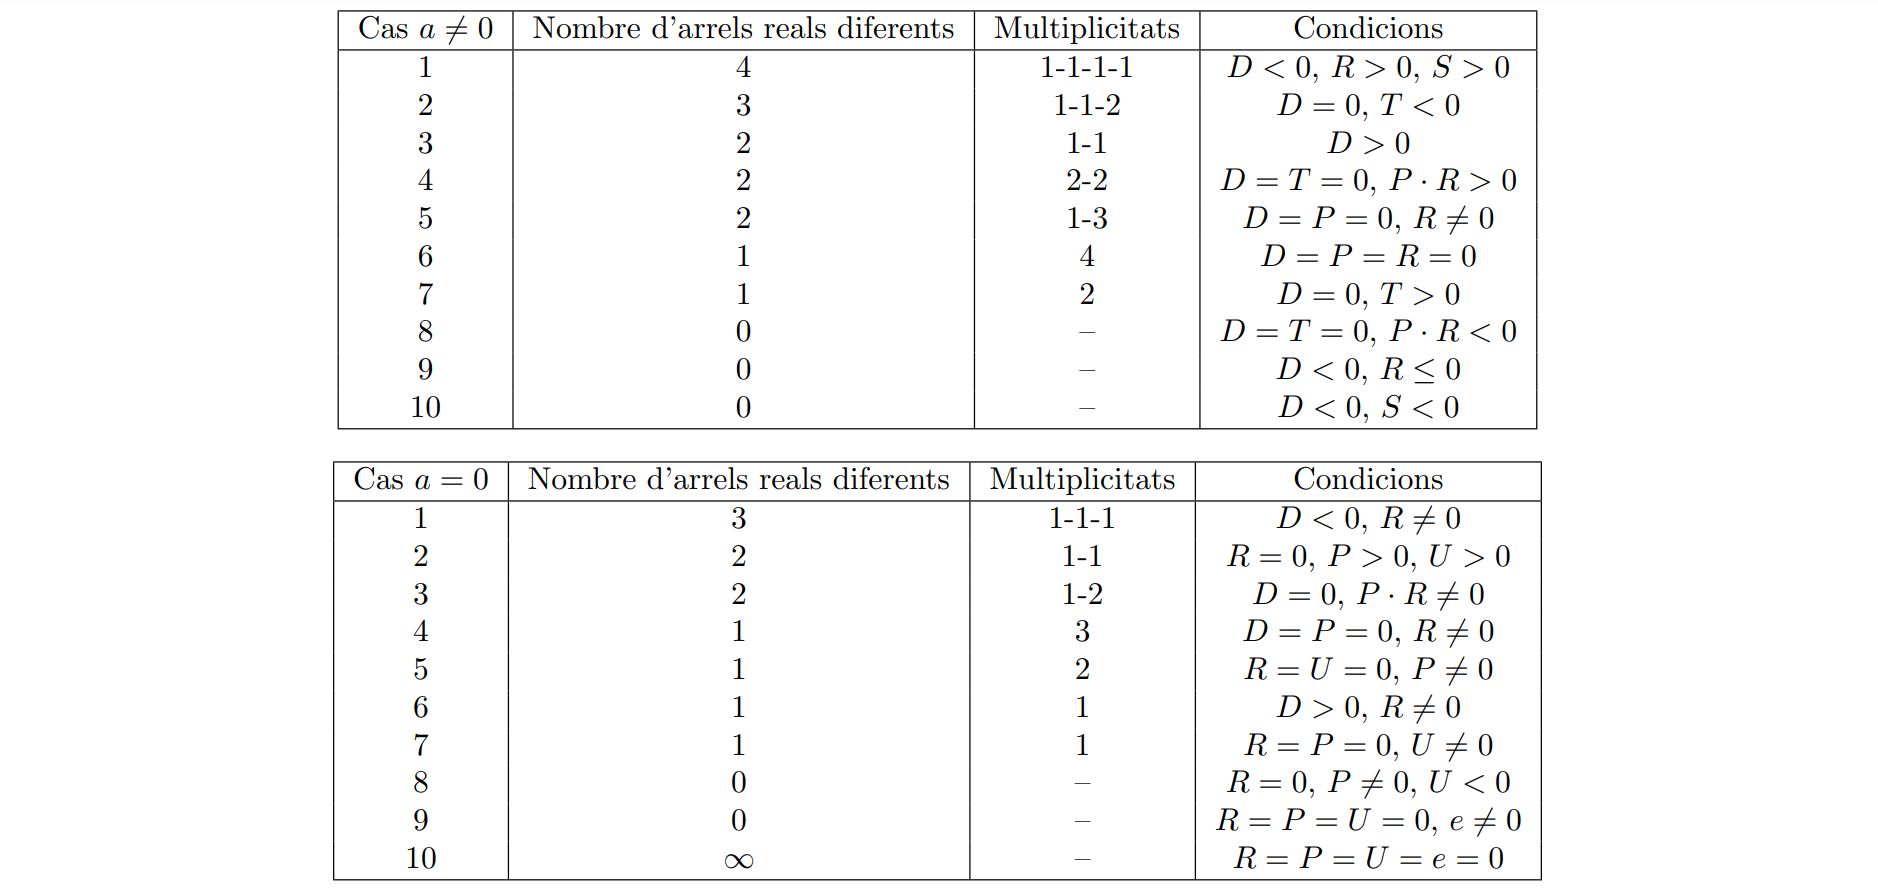
\includegraphics[width = 1 \textwidth]{Captura de pantalla 2022-05-05 160830.png}
    \label{fig:my_label}
\end{figure}\\
Com que el programa genera polinomis amb coeficients de forma aleatòria, segons una normal amb paràmetres (0,1), hi ha alguns casos que no cal contemplar (és a dir, que tenen probabilitat 0).
\\
També es pot veure que, en la taula, tenim informació redundant, de manera que es poden resumir les condicions i els càlculs dels discriminants per calcular només els imprescindibles.\\
\newpage
\hspace{-1.5em}Per tal de simplificar els càlculs, tenim en compte: \label{1}
\begin{itemize}
    \item [-] El cas $a=c$ (per a un $c$ donat) té probabilitat $0$, per lo que no cal usar les condicions de classificació de la taula $a=0$.
    \item [-] En no contemplar el cas $a=0$, no cal calcular el discriminant $U$ mencionat anteriorment.
    \item [-] Els casos $1$, $2$, $4$, $5$ i $6$ donen 4 arrels reals. El $5$ i $6$ es poden fusionar en la condició $D=P=0$.
    \item [-] Els casos $3$ i $7$ donen 2 arrels reals i 2 complexes.
    \item [-] Els casos $8$, $9$ i $10$ donen 4 arrels complexes.
\end{itemize}
Tenint en compte aquests punts, el primer esborrany del classificador va ser:

\small\begin{verbatim}
    if(disc[1]>0 || !disc[1]*disc[5]>0) goto both;
    if(disc[1]<0){
        if (disc[2] > 0 && disc[4] > 0) goto real;
        if(disc[4]<=0 || disc[2]<0) goto complex;
        goto out;
    }
    if(!disc[1]*!disc[5]){
        if(disc[0]*disc[4]<0) goto complex;
        if(disc[0]*disc[4]>0) goto real;
    }
    if(!disc[1]*!disc[0] || !disc[1]*disc[5]<0) goto real;
\end{verbatim}
On \texttt{disc[0]} = $P$, \texttt{disc[1]} = $D$, \texttt{disc[2]} = $S$, \texttt{disc[3]} = $Q$, \texttt{disc[4]} = $R$ i \texttt{disc[5]} = $T$.
\\
Durant el procés d'obtenció del primer model de filtratge vam tenir problemes classificant funcions que tenien 4 arrels reals degut a una equivocació a l'hora de redactar les condicions (en comptes de posar \texttt{disc[2] > 0 \&\& disc[4] > 0} vam posar \texttt{!disc[2] \&\& disc[4] > 0}) pel que tots els càlculs desquadraben.\\
Al adonar-nos de l'error i corretgir-lo ens vam adonar que aquella condició de manera exclusiva classificaba tots el polinomis de grau quatre amb arrels reals.\\
Deduírem que hi havia casos amb probabilitat 0 que no haviem identificat com a innecesaris, pel que una vegada ja teniem poques condicions, vam determinar, tant a prova i error com amb relacions lògiques) quines de les condicions que teniem eren innecesàries.\\
L'output que obteniem amb la primera versió correcte del classificador era similar a:
\begin{verbatim}
    Fraction of polynomials quadratic with 4 real roots: 0.245215
    Fraction of polynomials quadratic with 4 complex roots: 0.085308 
    Fraction of polynomials quadratic with 2 real roots and 2 complex roots: 0.669477 
\end{verbatim}
Una vegada vam provar quines eren condicions necesàries (les que mantenien el resultat correcte) vam finalitzar obtenint la següent cadena de \texttt{if} per classificar:
\begin{verbatim}
    if(discriminants[1] > 0) n_types[2]++;
    else{
      if (discriminants[4] > 0 && discriminants[2] > 0) n_types[0]++;
      else n_types[1]++;
    }
\end{verbatim}
On \texttt{discriminants[1] = D}, \texttt{discriminants[2] = S} i \texttt{discriminants[4] = R}.\\
Per tant, acabem concluïnt que les úniques restriccions necessàries per classificar són:
\begin{itemize}
    \item [-] $D > 0$: 2 arrels reals i dos arrels complexes
    \item [-] $D \leq 0$, $S > 0$ i $R > 0$: 4 arrels reals
    \item [-] $D \leq 0$, $S \leq 0$ o $R \leq 0$: 4 arrels complexes
\end{itemize}
Degut a aquesta reducció de les condicions, només ha sigut necessari calcular els discriminants $P$, $D$, $S$, $Q$ i $R$ (estalviant-nos així el càlcul de la $U$ i la $T$).
\\
També comentar, que s'ha decidit posar aquesta distribució de les comparacions degut a que és més probable obtenir 2 arrels reals i 2 complexes que només 4 reals; i és més probable obtenir 4 reals que 4 complexes.


\newpage
\section{Comprovacions de funcionament}\label{comprovacions}
Per asegurar el correcte funcionament del programa, aplicant el que hem analitzat en l'apartat \textcolor{blue}{\ref{desen_program}}, adjuntem ara un seguit de taules amb tota la informació obtinguda (aplicant varies vegades el programa generant polinomis de manera aleatòria):\\
Usant la comanda \texttt{./arrels}
\begin{table}[h]
    \centering
    \begin{tabular}{c||c|c|c}
        \textbf{Generació} & \textbf{$4$ arrels reals} & \textbf{$4$ arrels complexes} & \textbf{$2$ arrels reals i $2$ complexes} \\\hline\hline
        1 & 0.245181 & 0.085204 & 0.669615 \\\hline
        2 & 0.244983 & 0.085351 & 0.669666  \\\hline
        3 & 0.245044 & 0.085185 & 0.669771 \\\hline
        4 & 0.245058 & 0.085133 & 0.669808  \\\hline
        5 & 0.245034 & 0.085303 & 0.669663\\
        
    \end{tabular}
    \label{tab:my_label}
\end{table}\\
Usant la comanda \texttt{./arrels 1} i definint com \textbf{Tipus 1} els polinomis amb $4$ arrels reals, \textbf{Tipus 2} els polinomis amb $4$ arrels complexes i \textbf{Tipus 3} els polinomis amb $2$ arrels de cada (reals i complexes); obtenim la següent taula de generacions:
\begin{table}[h]
    \centering
    \begin{tabular}{c||c|c|c|c|c|c|c|c}
        \multirow{2}{*}{\textbf{Gen.}} & \multicolumn{2}{c|}{\textbf{Tipus 1}}  & \multicolumn{2}{c|}{\textbf{Tipus 2}} &  \multicolumn{2}{c|}{\textbf{Tipus 3}} & \multicolumn{2}{c}{\textbf{Others}} \\
        & \#Creats & Fracció & \#Creats & Fracció  & \#Creats & Fracció  & \#Creats & Fracció \\ \hline \hline
        1 & 4898321 & 0.244916 & 1705573 & 0.085279 & 13396106 & 0.669805 & 0 & 0.000000 \\\hline
        2 & 4896770 & 0.244838 & 1704272 & 0.085214 & 13398958 & 0.669948 & 0 & 0.000000 \\\hline
        3 & 4900629 & 0.245031 & 1702771 & 0.085139 & 13396600 & 0.669830 & 0 & 0.000000 \\\hline
        4 & 4900973 & 0.245049 & 1703550 & 0.085178 & 13395477 & 0.669774 & 0 & 0.000000 \\\hline
        5 & 4902916 & 0.245146 & 1704086 & 0.085204 & 13392998 & 0.669650 & 0 & 0.000000 \\
    \end{tabular}
    \label{tab:my_label}
\end{table}
\newpage
\hspace{-1.5em}Per tal de comprovar que el vostre programa funcioni correctament, podeu usar la comanda\\ \texttt{./arrels 1 10 0} i comprovar que l'output que us surt és igual a:\\
\begin{verbatim}
Extra information has been requested.
Number of samples changed.
Values of the seed changed.
Calculating...
End of the calculations.

----------------------------------------------------------------------------------
Number of polynomial functions of degree 4 generated: 10

Number of which has 4 real root: 1
Fraction of polynomials quadratic with 4 real roots: 0.100000 

Number of which has 4 complex root: 2
Fraction of polynomials quadratic with 4 complex roots: 0.200000 

Number of which has 2 real roots and 2 complex roots: 7
Fraction of polynomials quadratic with 2 real roots and 2 complex roots: 0.700000 
..................................................................................
Number of other cases: 0
Fraction of other cases: 0.000000 
----------------------------------------------------------------------------------
Time elapsed from the start to the end of the program: 0 ms
\end{verbatim}



\newpage
\section{Conclusions}
Finalitzem l'informe confirmant (a partir de les comprovacions de funcionament dutes a terme a l'apartat \textcolor{blue}{\ref{comprovacions}}) que el programa $arrels.c$ funciona de manera correcta, proporcionant les fraccions de polimonis quadràtics amb 4 arrels reals, 4 arrels complexes, i 2 reals 2 complexes.\\
Per tant, podem afirmar també que la funció \textbf{\textcolor{funcblue}{muller()}} funciona correctament, ja que depen únicament del correcte funcionament de la funció \textbf{\textcolor{funcblue}{Normal()}} a l'hora de generar els coeficients aleatoris.\\
\subsection{Informació adicional}
\begin{itemize}
   \item Responem a la pregunta: \textbf{ En les taules hi ha tots els casos possibles que es poden donar. Els necessiteu tots per la implementació? Per què? En cas negatiu, quins són supèrfluos?}\\
   Responem aquesta pregunta a l'apartat \textcolor{blue}{\ref{1}}.
   
   \item Responem a la pregunta: \textbf{Què vol dir la fila 10 de la taula cas $a=0$ quan diu que hi ha infinites arrels reals?}\\
   Si suposem $R=P=U=e=0$ obtenim que: 
   \begin{enumerate}
        \item $R=P=U=e=0$ ocurreix en el cas $a=0$ 
        \item $U=0 \Rightarrow 2\cdot d^2-3c\cdot0 \Rightarrow d=0$
        \item $P=0 \Rightarrow a\cdot0-4b\cdot0+3c^2=0 \Rightarrow c=0$
        \item $R=0 \Rightarrow b^2-a\cdot0=0 \Rightarrow b=0$
   \end{enumerate}
   Per tant, observem que tots els coeficients són $0$; es a dir, $\forall x\in\mathbb{C}, f(x) = 0$,\\ essent $f(x):= ax^4+4bx^3+6cx^2+4dx+e\in\mathbb{R}_4[X]$ (hi ha infinites solucions).
   
   \item  La complexitat dels mètodes són d'ordre lineal; és a dir, $O(n)$ (on $n$ és el nombre de mostres que volem que generi el programa).
   
   \item Aconsellem llegir la \textcolor{blue}{\href{https://www.overleaf.com/read/nxmjqvcfdtrt}{Pràctica 2}} per informació complementària sobre l'ús i les propietats del programa.
   
\end{itemize}

\end{document}
